
\begin{figure}
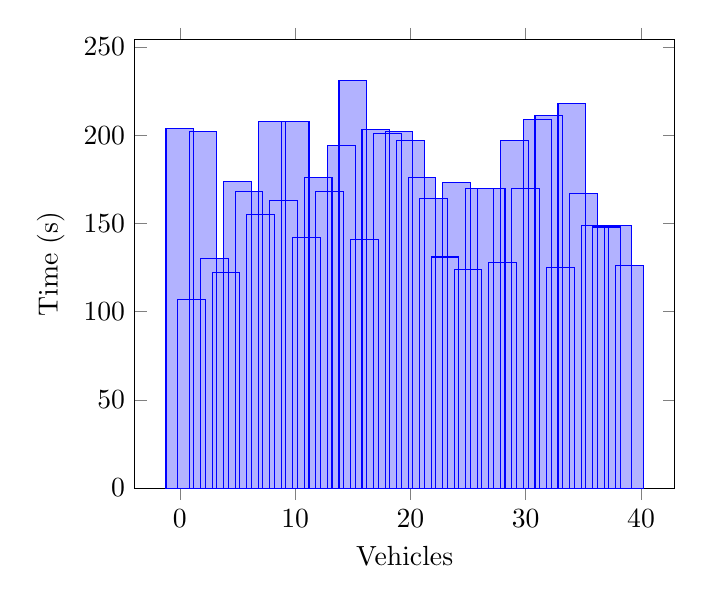
\begin{tikzpicture}
\begin{axis}[
legend style={anchor=west},
xlabel=Vehicles,
ylabel=Time (s),
ymin=0,
ybar,
]
\addplot coordinates {
(0, 204)
(1, 107)
(2, 202)
(3, 130)
(4, 122)
(5, 174)
(6, 168)
(7, 155)
(8, 208)
(9, 163)
(10, 208)
(11, 142)
(12, 176)
(13, 168)
(14, 194)
(15, 231)
(16, 141)
(17, 203)
(18, 201)
(19, 202)
(20, 197)
(21, 176)
(22, 164)
(23, 131)
(24, 173)
(25, 124)
(26, 170)
(27, 170)
(28, 128)
(29, 197)
(30, 170)
(31, 209)
(32, 211)
(33, 125)
(34, 218)
(35, 167)
(36, 149)
(37, 148)
(38, 149)
(39, 126)
};

\end{axis}
\end{tikzpicture}
\label{tik:0:1_S, 1_S.-60, 4_S, 5_S, 5_S.-30, 7_S, 7_S.-25, 11_S, 11_S.-50, 13_S, 15_N, 17_S, 17_S.-60, 19_V}
\caption{0 percent diving with GSC on route $1_S, 1_S.-60, 4_S, 5_S, 5_S.-30, 7_S, 7_S.-25, 11_S, 11_S.-50, 13_S, 15_N, 17_S, 17_S.-60, 19_V$}
\end{figure}
